Find the value of k such that 
\begin{align}
	6x^2 + 11xy - 10y^2 + x + 31y + k =0 \label{eq:solutions/13/6/eq:eq5}
\end{align}

represent pairs of straight lines.

From \eqref{eq:solutions/13/6/eq:eq5} we get,
\begin{align}
	\vec{V} &= \myvec{6 & \frac{11}{2} \\ \frac{11}{2} & -10}\\
	\vec{u} &= \myvec{\frac{1}{2}\\ \frac{31}{2}}\\
	f &= k
\end{align}
Compute the slopes of lines given by the roots of the polynomial $-10m^2 + 11m + 6$
\begin{align}
   i.e., m_i &= \frac{-b \pm \sqrt{- \mydet{\vec{V}}}}{c} \label{eq:solutions/13/6/eq:eq2} \\
   \implies m &= \frac{\frac{-11}{2} \pm \frac{19}{2}}{-10} \\ 
   \implies m_1 &= \frac{-2}{5}, m_2 = \frac{3}{2} 
\end{align} 
Let the pair of straight lines be given by 
\begin{align}
	\vec{n}_1^T\vec{x} = c_1 \label{eq:solutions/13/6/eq:n_1}\\
	\vec{n}_2^T\vec{x} = c_2 \label{eq:solutions/13/6/eq:n_2}
\end{align}
Here,
\begin{align}
	\vec{n}_1 &= k_1\myvec{-m_1\\1} = k_1 \myvec{ \frac{2}{5} \\ 1}  \label{eq:solutions/13/6/eq:n1val}\\
	\vec{n}_2 &= k_2\myvec{-m_2\\1} = k_2 \myvec{\frac{-3}{2} \\ 1} \label{eq:solutions/13/6/eq:n2val}
\end{align}
We know that, 
\begin{align}
	\vec{n}_1 * \vec{n}_2 = \myvec{a\\2b\\c} \label{eq:solutions/13/6/eq:n1n2}
\end{align}
Substituting \eqref{eq:solutions/13/6/eq:n1val} and \eqref{eq:solutions/13/6/eq:n2val} in the above equation, we get
\begin{align}
	k_1 \myvec{ \frac{2}{5} \\ 1} * k_2 \myvec{\frac{-3}{2} \\ 1} &= \myvec{6\\ 11\\ -10}\\
	\implies k_1k_2 &= -10
\end{align} 
By inspection, we get the values, $k_1 = 5, k_2 = -2$. Substituting the values of $k_1$ and $k_2$ in \eqref{eq:solutions/13/6/eq:n1val} and \eqref{eq:solutions/13/6/eq:n2val} respectively, we get
\begin{align}
	\vec{n}_1 &= \myvec{2 \\ 5} \label{eq:solutions/13/6/eq:n1}\\
	\vec{n}_2 &= \myvec{3 \\ -2} \label{eq:solutions/13/6/eq:n2}
\end{align}
Using Teoplitz matrix representation, the convolution of $\vec{n}_1$ with $\vec{n}_2$, is as follows:
\begin{align}
	\myvec{2 & 0 & 5\\ 5 & 2 & 0\\ 0 & 5 & 2}\myvec{3\\-2\\0} = \myvec{6 \\11 \\ -10} = \myvec{a \\ 2b \\ c}
\end{align}
Hence, $\vec{n}_1$ and $\vec{n}_2$ satisfies \eqref{eq:solutions/13/6/eq:n1n2}.
We have,
\begin{align}
	c_2\vec{n}_1 + c_1\vec{n}_2 &= -2\vec{u} \label{eq:solutions/13/6/eq:cneq}
\end{align}
Substituting \eqref{eq:solutions/13/6/eq:n1}, \eqref{eq:solutions/13/6/eq:n2} in \eqref{eq:solutions/13/6/eq:cneq}, we get
\begin{align}
 \myvec{2 & 3\\ 5 & -2}\myvec{c_2 \\ c_1} &= -2\myvec{\frac{1}{2} \\ \frac{31}{2}}
\end{align}
Solving for $c_1$ and $c_2$, the augmented matrix is,
\begin{align}
	\myvec{2 & 3 & -1\\ 5 & -2 & -31} &\xleftrightarrow[R_2 \leftarrow R_2 - 5R_1]{R_1 \leftarrow \frac{R_1}{2}} \myvec{1 & \frac{3}{2}  & \frac{-1}{2} \\ 0 & \frac{-19}{2} & \frac{-57}{2}} \\
	&\xleftrightarrow[R_1 \leftarrow R_1 - \frac{3}{2}R_2]{R_2 \leftarrow \frac{R_2}{-19/2}} \myvec{1 & 0 & -5\\0 & 1 & 3}
\end{align}
Hence we obtain,
\begin{align}
	c_1 = 3, c_2 = -5
\end{align}
We know that,
\begin{align}
	f = k = c_1c_2\\
	\implies \boxed{k = -15}
\end{align}
Hence the solution. Using \eqref{eq:solutions/13/6/eq:n_1} and \eqref{eq:solutions/13/6/eq:n_2}, the equation of pair of straight lines is given by,
\begin{align}
\myvec{2 & 5}\vec{x} &= 3\\
\myvec{3 & -2}\vec{x} &= -5
\end{align}
See Fig. \ref{fig:solutions/13/6/}


\begin{figure}[!ht] 
	\centering
	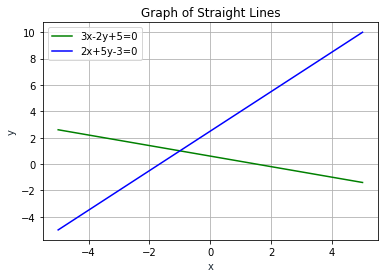
\includegraphics[width=\columnwidth]{./solutions/13/6/a6_graph.png}
	\caption{Plot of two straight lines.}
\label{fig:solutions/13/6/}
\end{figure}
